\section{Proposed Solution}
\label{sec:Solution}
In this Section we will address the components we will develop, capable of suggesting trustful actions to a generic autonomous agent. Our solution will be using the Repage architecture, described in Section \ref{subsubsec:Related work:Trust Models:Repage}, as it is the only implementable trust modelling architecture, that we found, created to be implementable, and not just a theoretical model. It's simplicity also goes in line with our goals of creating an easily comprehensible model, and developing a complete trust architecture is outside the scope of this project.

We will start with describing a trust model of the user in the Cognitive Trust Modelling Module (Section \ref{subsec:Solution:Trust Decision Making Module}), go on to the Trustful Action Suggestion Module (Section \ref{subsec:Solution:Trust Decision Making Module}) that will actually handle action suggestion, and finally talk about how they connect together and to the rest of a generic agent architecture.


\subsection{Cognitive Trust Modelling Module}
\label{subsec:Solution:Trust Assessment Module}
In this module we aim to create a trust representation of the user. The model must be able to represent the user's trust beliefs, while also provide an evaluation on how trustworthy is the agent in the eyes of the user. 

This module will represent the memory and detector components of the Repage architecture (Section \ref{subsubsec:Related work:Trust Models:Repage}). The concrete implementation for the beliefs is still under discussion, but our main candidate would be the \textit{BC}-Logic described in \ref{subsubsec:Related work:Trust Models:BDI + Repage} by Pinyol et al., \cite{Pinyol2009}.

\subsection{Trustful Action Suggestion Module}
\label{subsec:Solution:Trust Decision Making Module}
This module is still very roughly defined as no related work was found about this topic, so most work done in this module will be on experimenting what information can be extracted from the trust model. The main goal is to suggest actions that will either improve the strength of existing beliefs on the trust model, or improve the trust value on the agent, occupying the analyser component in the Repage architecture(Section \ref{subsubsec:Related work:Trust Models:Repage}).

\subsection{Putting it Together}
\label{subsec:Solution:Putting it Together}
The Trustful Action Suggestion Module is going to be directly dependent on the Cognitive Trust Modelling Module, as all decision making from the former module is going to be based on information from the latter module.
Both modules must be integrated with the agent in which we will evaluate the work with. Depending on the current state of the agent, a translation module may have to be created, to connect the main memories of the agent to the memories in Cognitive Trust Modelling Module. Additionally the Trustful Action Suggestion Module must also be added onto the planner component of the agent, so that the suggestions will be taken into account.
The overall architecture dependencies can be checked in Figure \ref{fig:arquitecture}. 


\begin{figure}[hbt]
	\centering
	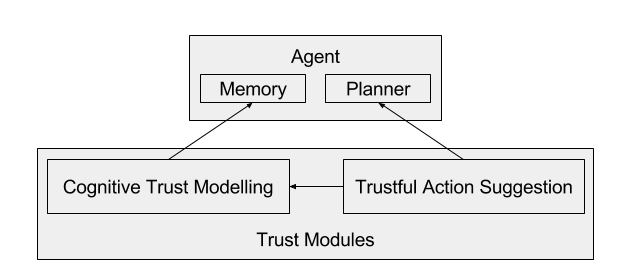
\includegraphics[width=\textwidth]{figures/arquitecture.png}
	\caption{Solution architecture schematic}
	\label{fig:arquitecture}
\end{figure}
